\subsubsection{Stelleinheit}
Um die Abwurfeinheit zum Ziel auszurichten, wird ein verstellbarer Mechanismus benötigt. Der Drehpunkt muss sich möglichst unter den Schwungrädern befinden, damit die Position des Abwurfes im Zentrum des Spielfeldes bleibt. Die Drehung wird durch einen Schrittmotor angesteuert. Die Wahl des Schrittmotors ist durch seine sehr exakte Ansteuerung ausgefal-len. Somit kann der Verstellwinkel, welcher von der Position des Zieles abhängt, genau eingestellt werden. Der Schrittmotor wird in der Abwurfeinheit angebracht und treibt die Bo-denplatte an, wodurch die Abwurfeinheit gedreht wird. Damit die Bauhöhe nicht zusätzlich erhöht wird, ist der Zahnkranz in die Bodenplatte integriert. Die Bodenplatte mit dem Zahn-kranz reicht nicht über die ganze Abwurfeinheit, damit die Masse möglichst klein gehalten werden kann. Der Schrittmotor ist nach dem folgenden Drehmoment von …Nm ausgelegt. Dies ist sehr klein, da nur der Reibungskoeffizient und die Normalkraft, welche vom Gewicht der Abwurfeinheit abhängt, das Moment erzeugen. Der Reibungskoeffizient wird durch die Lagerung klein gehalten. Die Lagerung erfolgt im Drehzentrum durch eine Hülse und im Endbereich der Abwurfeinheit durch zwei Kugelrollen, welche mit einem seitlichen Abstand angebracht sind. Dadurch ist auch die Gefahr eines Umkippens der Abwurfeinheit gesi-chert. Die Ansteuerung der Schrittmotoren erfolgt über den selbst konstruierten Controller. (Verlinkung zur Beschreibung der Motorentreiber)

\begin{figure}
	\centering
	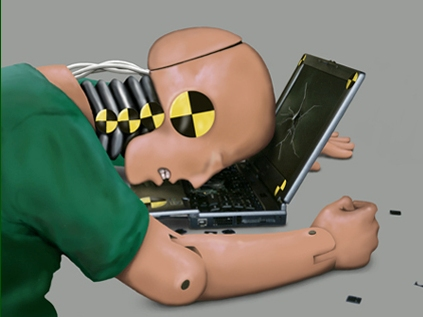
\includegraphics[width=0.9\textwidth]{Enddokumentation/CrashTestDummy.jpg}
	\caption{Grafik des Antriebes}
	\label{fig:Grafik des Antriebes}	
\end{figure}